\documentclass[aspectratio=169,14pt]{beamer}
\usetheme{htlpi}
\usepackage[utf8]{inputenc}

\title{Fireman's Friends}
%\subtitle{Untertitel}
\author{Denise Kohlhauser, Lisa Muhr}
\institute{5AHIF}
\titlegraphic{
\includegraphics[width=5cm]{Logo_Informatik.pdf}}
\date{29. April 2019}

\begin{document}
    \begin{frame}
        \maketitle
    \end{frame}
    
    \begin{frame}[t]{Aufgabenstellung}
        \begin{itemize}[<+->]
            \item Erstellung eines Online-Trainers
            \item Benutzerverwaltung
            \item Administrator-Bereich
            \item Statistikfunktion
            \item Responsive Design
        \end{itemize}
    \end{frame}
    
    \begin{frame}[t]{Zweispaltige Folie}
        \begin{columns}[T]
            \begin{column}{0.5\textwidth}
                \begin{itemize}
                    \item Text
                    \item Text
                        \begin{itemize}
                            \item Text
                            \item Text
                                \begin{itemize}
                                    \item Text
                                    \item Text
                                    \item Text
                                \end{itemize}
                            \item Text
                        \end{itemize}
                    \item Text
                \end{itemize}
            \end{column}
            \begin{column}{0.5\textwidth}
                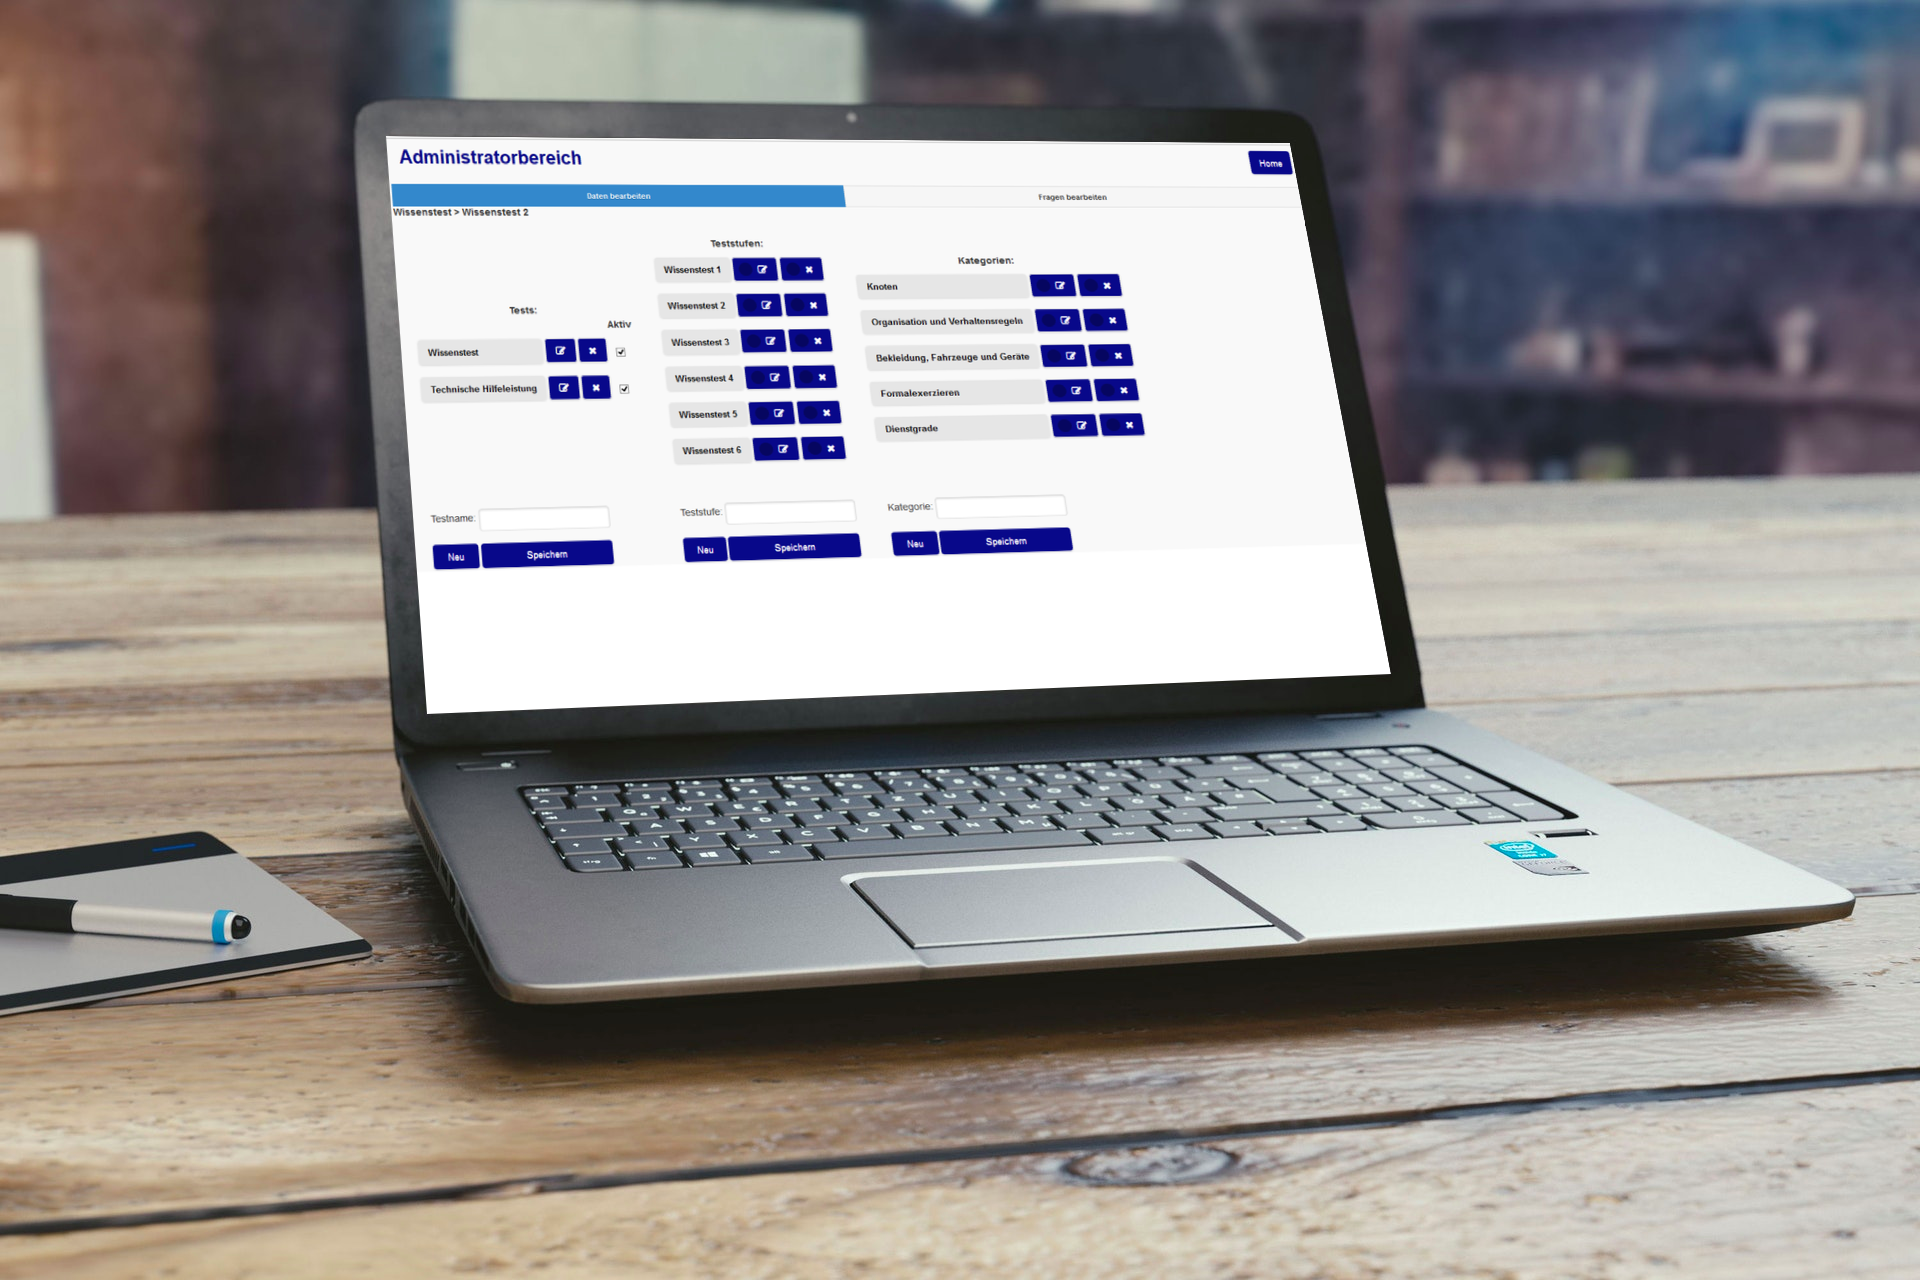
\includegraphics[height=0.5\textheight]{FiremansFriends-2-mockup.png}
            \end{column}
        \end{columns}
    \end{frame}
    
    \begin{frame}[part]{Responsive Design}
        \framesubtitle{Individueller Teil – Lisa Muhr}
    \end{frame}
    
    \begin{frame}[focus]
        \usebeamerfont{callout}
        Demo
    \end{frame}
    
    \begin{frame}[focus]
        Zusatzfolien
    \end{frame}

    \begin{frame}[t]
        \begin{tikzpicture}[remember picture,overlay]
                \node[at=(current page.center)] {
                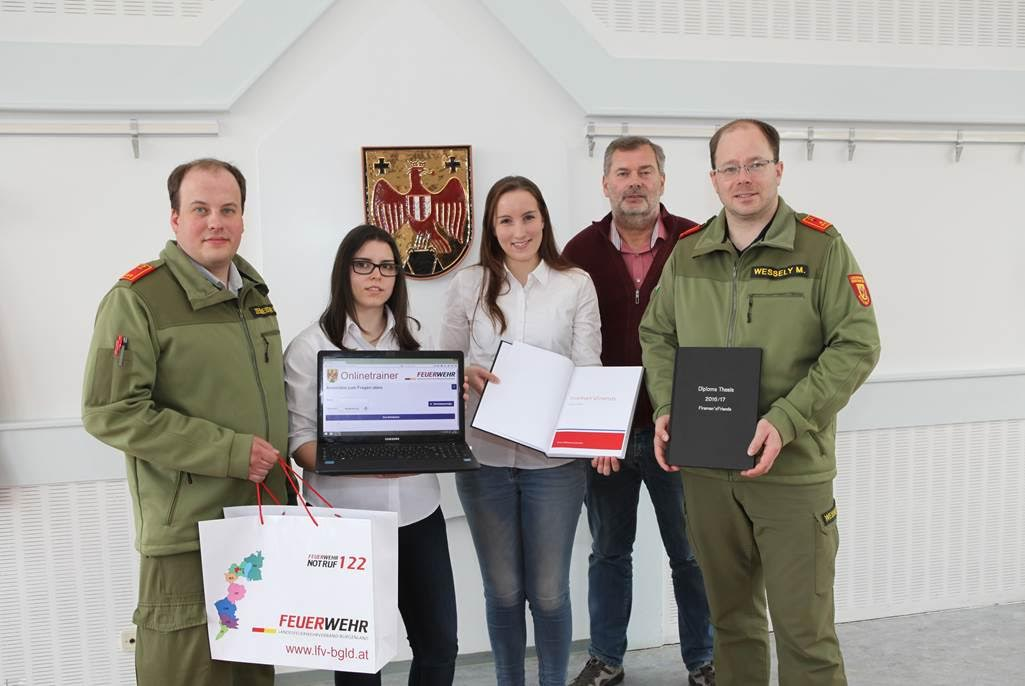
\includegraphics[keepaspectratio,
                     width=\paperwidth]
                     {FiremansFriends-4.jpg}
                };
        \end{tikzpicture}
    \end{frame}
\end{document}
